% !TeX TS-program = xelatex

\documentclass{resume}
\usepackage{graphicx}                                                           
\usepackage{float} 
\ResumeName{刘锦帆}

\begin{document}

% % TODO: Figure Insertion
% \usepackage{wrapfig}
% \begin{wrapfigure}{r}{4cm} 
%     \centering
%     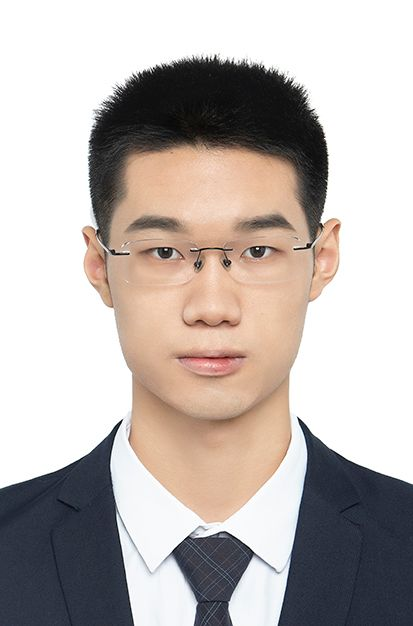
\includegraphics[width= 0.5in]{pic.png}
% \end{wrapfigure}

\ResumeContacts{
    (+86) 15008278732,%
    \ResumeUrl{mailto:3020202184@tju.edu.cn}{3020202184@tju.edu.cn},%
    \\ 
    \ResumeUrl{https://chrisvicky.github.io/}{chrisvicky.github.io} \footnote{下划线内容包含超链接。},%
    \ResumeUrl{https://github.com/ChrisVicky}{github.com/ChrisVicky}%
    }

    \ResumeTitle

    \section{教育经历}
    \ResumeItem
    [天津大学|本科]
    {天津大学}
    [\textnormal{计算机科学与技术|} 本科]
    [2020.09—2024.06(预计)]


    \section[技术能力]{技术能力\protect}
    \begin{itemize}
        \item \textbf{编程语言}: 编程不受语言限制: C/C++, Python, SQL, Java, Golang, Lua, Rust, Shell, Matlab, Tex等
        \item \textbf{工作流}: Arch Linux, Shell, (Neo)Vim, Git, GitHub, IDEA(SpringBoot)等
        \item \textbf{后端}: Java (SpringBoot), Golang (GORM), Python (Flask), SQL, Docker, Redis, nginx, WASM 等
        \item \textbf{科研}: 分布式无人机集群控制技术, ROS, 机器视觉, Wi-Fi 定位, 多模态感知, PyTorch 机器学习等
    \end{itemize}

    \section{项目经历}

    \ResumeItem{天津大学•天外天工作室}
    [后端组组长•\ResumeUrl{https://github.com/ChrisVicky/52Hz}{“52Hz”}开发与维护]
    [2021.03-2021.05] 

    \begin{itemize}
        \item \textbf{独立完成}数据库以及业务逻辑、核心匹配算法的重新设计与实现
        \item \textbf{协调}其他组开发人员切换新的 API 以及产品测试,确保项目准时在 520 上线
    \end{itemize}

    \ResumeItem{天津大学•天外天工作室}
    [后端组组长•“青年湖底”维护与重构]
    [2022.06 - Now] 

    \begin{itemize}
        \item \textbf{组织} 三位开发将“青年湖底(校内论坛)”从 Golang 的 GORM 框架 重构到 Java 的  SpringBoot 框架
        \item \textbf{负责} 主要的维护工作,包括补丁的 Java 和 Golang 版本代码的设计与实现以及服务器维护问题
    \end{itemize}

    \ResumeItem{天津大学•计算机网络课程}
    [\ \ResumeUrl{https://github.com/ChrisVicky/TJU-2022-Socket-Computer-Network-Lab}{基于 socket 接口实现 C 的 server }\footnote{最终报告99分}]
    [2022.04.14]

    \ResumeItem{天津大学•计算机网络实践}
    [\ \ResumeUrl{https://github.com/ChrisVicky/TJU-2022-TCP-Computer-Network-Lab}{使用 UDP 实现 TCP 可靠传输协议}\footnote{100分}]
    [2022.10.19]

    \section{科研经历}

    \ResumeItem{胡清华课题组}
    [动态环境下去中心化无人机群的自适应群体决策算法研究\textbf{(国家级)}]
    [2021.09 - 2022.09]
    \begin{itemize}
        \item \textbf{基本实现了} ROS 系统驱动的多架四旋翼无人机集群的分布式控制与同步、求解局部最优解的模型
        \item 手工制造并驱动多架无人机,同时进行试飞等实验,开创课题组的真机实验先河
        \item \textbf{负责} 将研究成果整理并\textbf{组织} 团队“Z.E.U.S: 灾害应急无人机蜂群系统”参加 “互联网+” 等比赛获金奖
    \end{itemize}

    \ResumeItem{佟鑫宇课题组}
    [视觉及 Wi-Fi 地图同步与感知技术\textbf{(小组长)}]
    [2022.09 - Now]
    \begin{itemize}
        \item \textbf{协助}课题组博士生验证了 LSTM 在 RFID 系统定位预测模型中的 PyTorch 以及 Matlab 实现上的效率及性能差异  
        \item \textbf{负责}课题“视觉及Wi-Fi多模态的地图同步与感知”的主要调研、代码设计与实现,主要技术栈: libfreenect2 开源库, libssh, SLAM, OpenCV 库, YOLOv5 模型, socket 框架, cURL 库, Flask 框架
    \end{itemize}

    \ResumeItem{天津大学•深度学习课程}
    [\ \ResumeUrl{https://github.com/ChrisVicky/TJU-2023-Deep-Learning-Report/tree/main}{改进 Vision Transformer}\footnote{90分}]
    [2023.01.15]

    \ResumeItem{天津大学•机器视觉课程}
    [\ \ResumeUrl{https://github.com/ChrisVicky/TJU-2023-Computer-Vision-Final}{基于Optical Flow 的 Control Net 控制模块}\footnote{尚未出分}]
    [2023.04.15]


    \section{获奖情况}
    \ResumeScholar{苏州育才奖学金(1万元)}[2022.11.15]
    \ResumeScholar{2022 年“挑战杯”中国银行天津市大学生创业计划竞赛(金奖)}[2022.07.01]
    \ResumeScholar{第八届中国国际“互联网+”大赛天津赛区主赛道(金奖)}[2022.09.09]
    \ResumeScholar{天津大学 2021 年三好学生}[2021.10.31]
    \ResumeScholar{第二届川蜀模范学子助力奖(科技创新突出成果奖•6万元)}[2020.07.14]
    \ResumeScholar{全国青少年信息学奥林匹克联赛复赛提高组四川赛区(一等奖)}[2018.12.15]
    \ResumeScholar{成都市第三十一届青少年科技创新大赛(英才奖)}[2015.12.04]



    \section{个人总结}

    \begin{itemize}
        \item 可以使用英语进行工作交流,阅读英文书籍及文档
        \item Arch Linux 忠实用户,较为丰富的软件开发和“折腾”经验,写过多线程程序
        \item \textbf{GPA: 3.78/4.0},在保持良好 GPA 的情况下参与多个工程、科研项目。同时积极参与公益活动,拓宽视野。了解并学习 \ResumeUrl{https://suckless.org/}{suckless} 等软件设计哲学
            % \begin{itemize}
            %     \item[] \begin{itemize}
            %             \item[•] 在天津大学\textbf{“天外天工作室”}任\textbf{后端组组长}
            %             \item[•] 在\textbf{“胡清华课题组”}参与\textbf{国家级大创“动态环境下去中心化无人机群的自适应群体决策算法研究”}
            %             \item[•] 在\textbf{“天津大学佟鑫宇课题组”}任\textbf{科研助手}, 负责\textbf{“视觉 及 Wi-Fi 地图同步与感知技术”} 小组
            %         \end{itemize}
            % \end{itemize}
        \item \textbf{英语:托福 104} \footnote{2023年1月14日考试(阅读 26,听力 26,口语 25,写作 27)}

    \end{itemize}


\end{document}
